\section{Evaluation}\label{sec:eval}

% We evaluate \thecontrib against baselines from the literature, namely \texttt{FedAvg}~\cite{mcmahan_communication-efficient_2017}, and \texttt{FoolsGold}~\cite{fung_limitations_2020}.
% We do these tests on a set of heterogeneous intrusion detection datasets~\cite{sarhan_standardfeatureset_2021} with a set of various attack scenarios (see \Cref{sec:eval.methodo.scenarios,sec:eval.results.attacks}).

\subsection{Methodology and setup\label{sec:eval.methodo}}
\subsubsection{Datasets\label{sec:eval.methodo.datasets}}
While most research on \glspl{fids} rely on splitting a single dataset among participants,
\citet{sarhan_standardfeatureset_2021} recently proposed a standardized feature set for flow-based \glspl{ids}. 
Furthermore, they converted four known \gls{ids} datasets to this format: UNSW-NB15~\cite{moustafa_unsw-nb15_2015}, Bot-IoT~\cite{koroniotis_towards_2019}, ToN\_IoT~\cite{moustafa_federatedtoniot_2020}, and CSE-CIC-IDS2018~\cite{sharafaldin_toward_2018}. 
This uniform feature set enable heterogeneous participants to source data from independently generated datasets~\cite{popoola_federated_2021,de_carvalho_bertoli_generalizing_2023}, a more realistic situation for \gls{fids}. 
We conduct our experiments on the ``sampled'' version which contain 1000000 samples per dataset~\cite{layeghy_generalisability_2022}. 
Like \citet{de_carvalho_bertoli_generalizing_2023}, we remove source and destination IPs and ports.
We then use one-hot encoding on the categorical features (both in the sample and labels), and finally apply min-max normalization to give all features the same importance in model training.


\subsubsection{Setup and reproducibility\label{sec:eval.setup}}
% As the literature shows a lack of reproducibility in both \gls{ml} and \gls{ids}, we emphasize making each of our experiments reproducible.
We implement \thecontrib and the comparison baselines using TensorFlow and the \gls{fl} framework Flower~\cite{beutel_flower_2020} on a NixOS server.  
The code for all experiments can be found online\footnote{Available at \codeurl}, with configuration and seeds for each considered baseline and evaluation scenario. 
We also provide lock files to enable anyone to reuse the same software version as in this paper.
% Ce serait bien de dire qu'on utilise Nix et qu'en 
% To evaluate its performance, we implement \thecontrib and the comparison baselines using TensorFlow 2.11 and the \gls{fl} framework Flower~\cite{beutel_flower_2020} (1.4.0).
% The experiments are done on a single NixOS server running Linux kernel 6.1.15, Python 3.10, and Poetry 1.3.2 for environment and package management.
% We provide all configurations\footnote{\codeurl} for anyone to reproduce said environment.
% The server has two AMD EPYC 7552 (192 cores total), 2 Nvidia Tesla T4 GPUs, and 768~GB of RAM. 

\subsubsection{Local algorithm\label{sec:eval.setup.local}}
Each client is equipped with a \gls{dl} \gls{mlp} model, we reuse the hyperparameters used by \citet{popoola_federated_2021}: they can be found in \Cref{tbl:hyperparameters}. 
% We also reproduce their results in \Cref{tbl:popoola_cross}.
% showing low performance when training the model on one dataset, and evaluating it on another.
% This supports the assumptions behind the cross-evaluation proposal, where the differences between the evaluation results can be used to estimate the similarity between the local data distribution.
% Train on one dataset / test on the others
% Takeaway : 
% - 
\subsubsection{Evaluation scenarios\label{sec:eval.methodo.scenarios}}

We implement the threat model defined in \Cref{sec:problem.threat} using label-flipping on the one-hot encoded classes, meaning that the label vector would go from $[0,1]$ to $[1,0]$ on a poisoned sample.
The \emph{stealthiness} of attackers is implemented as the proportion of the targeted samples that are poisoned.
For example, a \emph{stealth} attacker poisons 10\% of his target, whereas a \emph{loud} attacker selects 100\%.
The target depends on the type of attack: all sampled if untargeted, or malicious samples from a specific class in the case of targeted attacks.
To implement targeted attacks, similar to \citet{ma_shieldfl_2022}, we relabel a specific class of attack on the attacker.  
However, instead of relabeling the targeted class with another random class (\eg, relabeling "DoS" as "Reconnaissance"), we label the targeted attack class as benign since clients work on a binary classification task.

To distinguish the effect of the attack from the performance of the \gls{dl} model, we choose attacks that have high detection rates using \texttt{FedAvg}.
We also avoided the classes that had the most occurrences in each dataset, as we believe that their poisoning could leave a bigger footprint that would ease the detection. 
Specifically, this means "Bruteforce" in CSE-CIC-IDS2018, "XSS" in ToN\_IoT, and "Reconnaissance" in both Bot-IoT and UNSW-NB15.
For the rest of the experiments, and unless stated otherwise, the attacks will take place on BoT-IoT on label ``Reconnaissance''. 

Chosen attack for each dataset are exposed in \Cref{tab:targeted_attack}. 
In this table, the detection rate has been computed with \texttt{FedAvg} on data from a single dataset.  
We strived to select attacks that were well detected in centralized learning to make the effect of the attack more explicit. 

\begin{table}[]
%\end{minipage}\\
%
%\begin{minipage}{.7\textwidht}
    \centering
    \begin{tabular}{l|rrrr}
        \toprule % ---------------------------------
        \textbf{Models} & \multicolumn{4}{c}{\textbf{F1-Scores}} \\
                        & CIC-IDS & NB15 & ToN\_IoT & Bot-IoT \\
        \midrule % ---------------------------------
          CIC-IDS & \textbf{0.961787} &    0.002723 &  0.524219 &  0.680166 \\
          NB15 & 0.108913 &    \textbf{0.947204} &  0.009875 &  0.655943 \\
          ToN\_IoT & 0.211792 &     0.41938 &  \textbf{0.966679} &   0.08151 \\
          Bot-IoT & 0.158477 &    0.017188 &  0.703195 &  \textbf{0.999483} \\
        \bottomrule % ---------------------------------
    \end{tabular}
    \bigskip
    \caption{Cross evaluation (F1-score) on the full datasets.
    Each model (rows) is trained on 80\% of his dateset during 10 epochs, and then evaluated on each test set (columns).
    The train/test partitions are the same among tests.
    }
    \label{tbl:popoola_cross}
\end{table}
% \end{minipage}      
%\hfill
\begin{table}[]
% \begin{minipage}{.4\textwidth}
    % \centering
    \begin{subtable}{.45\linewidth}
    \centering
    \begin{tabular}{l|l}
        \toprule % ------------------------------------
        \multicolumn{2}{c}{Model hyperparameters} \\
       \midrule % ---------------------------------
         Learning rate & 0.0001 \\
        Batch size & 512 \\
        Hidden layers activation & ReLU \\
        Output layer activation & Sigmoid \\
        \# Input features & 49 \\
        \# Hidden layers & 2 \\ 
        \# Neurons (hidden layers) & 128 \\
        Optimization algorithm & Adam \\
        Loss function & Binary cross-entropy \\
        Number of local epochs & 10 \\
        \bottomrule % ---------------------------------
    \end{tabular}
    \end{subtable}%
    \begin{subtable}{.45\linewidth}
    \centering
    \begin{tabular}{l|l}
        \toprule % ---------------------------------
        \multicolumn{2}{c}{Clustering hyperparameters}\\
        \midrule % ---------------------------------
        Distance measured & Cosine~similarity (Eq.~\ref{eq:cosin_sim}) \\
        Hierarchical clustering & 1/4th of the mean \\
        Threshold &  initial inter-distance\\
        Cross-evaluation metric & F1-Score \\
        \midrule % ---------------------------------
        \multicolumn{2}{c}{Reputation hyperparameters}\\
        \midrule % ---------------------------------
        Number of classes & 10000 \\
        History parameter $\lambda$ & 0.3 \\ 
        Cross-evaluation metric & F1-Score \\
       \bottomrule % ---------------------------------
    \end{tabular}
    \end{subtable}
    
    \label{tbl:hyperparameters}
    \caption{Hyperparameters}


% \end{minipage}      
\end{table}


\subsubsection{Metrics\label{sec:eval.methodo.metrics}}

\thecontrib already produces evaluation metrics at each round thanks to the cross-evaluation scheme.
These metrics are related to the model performance based on the validation set.
The same evaluation methods are then used on a common testing set (to each initial client dataset) and aggregated to evaluate the approach.
Specifically, these metrics include accuracy, precision, recall, fallout, miss rate, and f1-score.
The same metrics are used for the other baselines.
We use the Rand index to measure the ability of \thecontrib to cluster clients correctly.
The Rand index compares two partitions from a group of participants by checking participants that are paired together in one of the partition are also paired together in the other partition. 
A Rand index of 1.0 means that both distributions are identical.

Then, following the methodology used in \texttt{FoolsGold}, we measure the \emph{attack success rate} as the percentage of samples that have been misclassified by the resulting global model.
For targeted attacks, the success rate is expressed as the mean of the miss rates of benign clients on the targeted attack classes.
Since untargeted attacks focus on impacting the classification by poisoning all labels (including benign samples), we chose the mean of the misclassification rates (\ie $1-accuracy$) of benign clients.

Finally, we exclude execution-related metrics such as training time, CPU overhead, or bandwidth consumption.
We leave the feasibility of \thecontrib to future works, and emphasize on its ability to maintain high accuracy.


\subsubsection{Baselines\label{sec:eval.setup.base}}

To position \thecontrib, we compare it with two existing \gls{fl} algorithms, namely \texttt{FedAvg}~\cite{mcmahan_communication-efficient_2017} and \texttt{FoolsGold}~\cite{fung_limitations_2020}.
We implement \texttt{FedAvg} to highlight the existing issues with statistical heterogeneity, using the setup provided by Flower\footnote{\url{https://github.com/adap/flower/blob/main/src/py/flwr/server/strategy/fedavg.py}}.
Note that without attackers, in the specific use case considered in this paper, \thecontrib can be assimilated as a per-distribution clustered \texttt{FedAvg} setup, just like the work of \cite{ye_pfedsa_2023}.

The extensive results in \Cref{fig:trustfids_accuracy_missrate_distribution} show the effectiveness of \thecontrib in most considered scenarios.
Yet, we also evaluate \thecontrib against \texttt{FoolsGold}, to highlight its ability to compare with Sybil-focused mitigation strategies, while remaining efficient otherwise, by combining clustering and reputation system.
\texttt{FoolsGold} was originally implemented on \texttt{FedSGD}, where each client uploads gradients. %, \ie the results of a step of \gls{gd}. 
%In \texttt{FedAvg}, clients execute the \gls{gd} algorithm $\mathcal{E} \times \lceil |d_i| / \beta \rceil$ times, depending on the number of epochs $\mathcal{E}$ and the batch size $\beta$ (see \Cref{sec:bg.fl}).
However, the authors note that from the perspective of their aggregator, comparing the cosine similarity of gradients or model updates has no impact on \texttt{FoolsGold}~\cite{fung_limitations_2020}.
Therefore, we use their provided \gls{dl} implementation\footnote{\url{https://github.com/DistributedML/FoolsGold/tree/master/deep-fg}}, and adapt it to model updates.
To stay true to the purpose of \texttt{FoolsGold}, and avoid losing information by comparing the models themselves, we use the difference between the uploaded model $\w$ and the last global model $\wbar[][r-1]$.
This is equivalents to the sum of the gradients if they were aggregated at each epoch, expressed as:
\begin{equation}\label{eq:gradients}
    \w - \wbar[][r-1] = \sum_{e=1}^\mathcal{E} \eta \nabla \lambda(w,d_i).
\end{equation}
%TODO le delta à l'envers moi j'ai pas compris

\subsection{Results\label{sec:eval.results}}

In these sections, we review the performance of \thecontrib concerning (a) its reaction to data poisoning attacks (\Cref{sec:eval.results.attacks}), and (b) how it compares with relevant baselines (\Cref{sec:eval.results.baselines}).
Finally, we evaluate independently the building blocks of the architecture in \Cref{sec:eval.results.cluster,sec:eval.results.reput}.

\begin{table}[]
% \begin{minipage}{.56\textwidth}
    \centering
        \caption{Accuracy is computed over all samples. Miss Rate is in percent, on targeted attacks it is computed only over the targeted classes, while on untargeted attacks it is computed over all classes from the attacked dataset.\label{tbl:accuracy_missrate_results}}
    \begin{tabular}{ll|cccccc}
        \toprule % ---------------------------------
        \multicolumn{2}{c}{\multirow{2}{*}{\textbf{Attack type}}} &
        \multicolumn{2}{c}{\textbf{\thecontrib}} &
        \multicolumn{2}{c}{\textbf{\texttt{FoolsGold}}} &
        \multicolumn{2}{c}{\textbf{\texttt{FedAvg}}} \\
        & & Acc & Miss & Acc & Miss & Acc & Miss  \\
        \midrule % ---------------------------------
        \multirow{4}{*}{\rotatebox[origin=c]{90}{\textbf{Targeted}}} & benign & \textbf{99.07} & \textbf{0.00} & 55.44 & 5.16 & 82.68 & 9.19 \\
        & lone & \textbf{99.06} & \textbf{0.00} & 60.51 &  93.82 & 77.38 & 21.45\\
        & Minority of byzantine & \textbf{98.96} & \textbf{0.00} & 54.64 & 2.97 & 78.48 & 16.59\\
        & Majority of byzantine & 98.28 & 73.39 & 85.10 & \textbf{8.10} & 79.40 & 18.78\\
        \midrule % ---------------------------------
        \multirow{4}{*}{\rotatebox[origin=c]{90}{\textbf{Untargeted}}} & benign & \textbf{99.07} & \textbf{1.82} & 55.44 & 19.28 & 79.49 & 5.09\\
        & lone & \textbf{98.96} & \textbf{2.03} & 49.56 & 72.29 & 78.38 & 16.48 \\ 
        & Minority of byzantine & \textbf{98.98} & \textbf{2.04} & 49.67 & 17.57 & 72.47 & 19.97 \\
        & Majority of byzantine & \textbf{98.96} & \textbf{2.21} & 69.09 & 68.24 & 81.87 & 19.20 \\
        \bottomrule % ---------------------------------
    \end{tabular}

    

%\end{minipage}      
\end{table}
%TODO y a un problème de mise en page avec ce tableau

\subsubsection{Resistance to attacks\label{sec:eval.results.attacks}}
\Cref{tbl:accuracy_missrate_results} presents the effect of the poisoning with varying number of attackers on the different baselines. 
Since we mostly want to know if benign participants can be poisoned by attackers, we strip attackers from the results and only keep benign participants.  
We then show the average accuracy of all benign participants.
%TODO pk de l'italique sur le miss ici ? 
The \emph{Miss} column is the average miss rate of participants as exposed in \Cref{sec:eval.methodo.metrics}.
A complete statistic overview of these results for \thecontrib is  visually exposed in \Cref{fig:trustfids_accuracy_missrate_distribution}.
For \thecontrib we can see that targeted attacks fail when attackers are a minority: the miss rate does not increase compared to the benign case.
The tipping point is when attackers outnumber legitimate participants: here, a majority of the targeted labels are misclassified. 
We can also see that the mean accuracy decreases with the number of attackers. Since we work with a fixed amount of data for each dataset, introducing attackers reduces the amount of data available for benign participants, which decreases their performance. 
We believe the same effect applies for the untargeted attack type, as untargeted attacks are easier to detect and are thus separated from benign for the aggregation (see \Cref{sec:eval.results.reput,sec:eval.results.cluster}).

\begin{figure}
  \centering 
  \begin{subfigure}{0.45\columnwidth}
    \centering 
    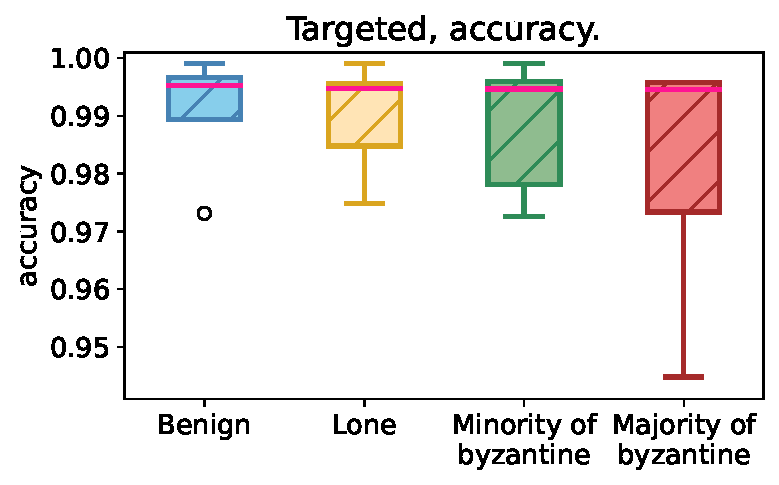
\includegraphics[width=\linewidth]{figures/poisoning/trusfids_targeted_acc_all_distibutions.pdf}    \caption{Targeted, accuracy.}
    \label{fig:trusfids_targeted_acc_all_distibutions}
  \end{subfigure}
  \begin{subfigure}{0.45\columnwidth}
    \centering 
    \includegraphics[width=\linewidth]{figures/poisoning/trusfids_untargeted_acc_all_distibutions.pdf}    \caption{Untargeted, accuracy.}
    \label{fig:trusfids_untargeted_acc_all_distibutions}
  \end{subfigure}
    
    \begin{subfigure}{0.45\columnwidth}
    \centering 
    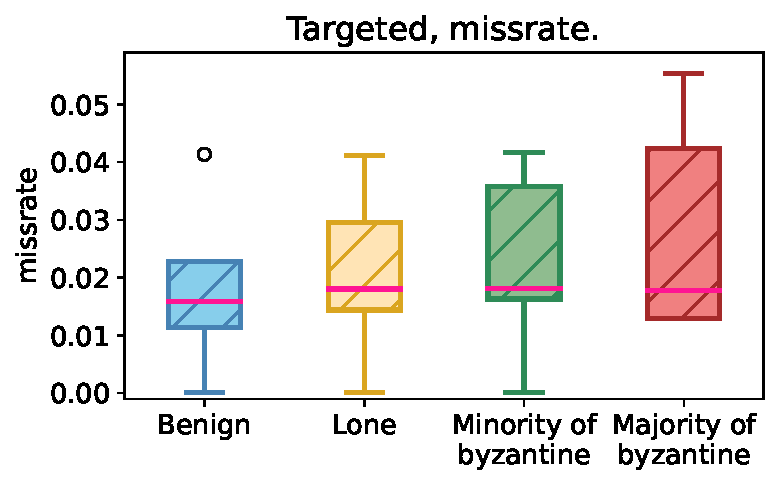
\includegraphics[width=\linewidth]{figures/poisoning/trusfids_targeted_missrate_all_distibutions.pdf}    \caption{Targeted, missrate.}
    \label{fig:trusfids_targeted_missrate_all_distibutions}
  \end{subfigure}
   \begin{subfigure}{0.45\columnwidth}
    \centering 
    \includegraphics[width=\linewidth]{figures/poisoning/trusfids_untargeted_missrate_all_distibutions.pdf}    \caption{Untargeted, miss rate.}
    \label{fig:trusfids_untargeted_missrate_all_distibutions}
  \end{subfigure}
  \hfill
  \caption{Statistical overview of \thecontrib's miss rates and accuracies in different attack scenarios.}
  \label{fig:trustfids_accuracy_missrate_distribution}
  
\end{figure}

\subsubsection{Baseline comparison\label{sec:eval.results.baselines}}

As we can see in \Cref{tbl:accuracy_missrate_results}, \texttt{FoolsGold} isn't adequate for practical \gls{niid} use cases, where groups of participants sharing similar distributions coexist. 
Benign participants coming from the same datasets sometimes show too much similarity, and end up being penalized. 
In the \emph{lone attack} scenario, benign models coming from the targeted dataset, in this case Bot-IoT, are all penalized.
It leads to a remarkably low detection rate on attacks coming from this dataset. 
In the Byzantine scenario with a \emph{minority} of attackers, only participants from the BoT-IoT dataset are kept, while those coming from other datasets are discarded. This leads to a model that is specialized on this dataset, and thus shows great results on the targeted class but an accuracy worse than \texttt{FedAvg} overall.
Finally, in the targeted Byzantine scenario with a \emph{majority} of attackers, malicious participants are dropped and all benign are kept, leading to slightly better results than a benign \texttt{FedAvg}.
% pathological non-IID inadequate for intrusion detection (benign + attack necessary), fools gold doesn't perform well in this setting either.


\subsubsection{Clustering\label{sec:eval.results.cluster}}

As detailed in \Cref{sec:archi.cluster}, the first goal of the clustering is to regroup similar participants to limit the impact of heterogeneity. 
From an experiment perspective, this means that participants whose data comes from the same dataset must be grouped together. 

In ~\Cref{fig:rand_clustering} we use the Rand index defined in \Cref{sec:eval.methodo.metrics} to compare the partition given by the clustering algorithm over several attack scenarios against two partitions of reference. 
In the first partition, we exclude attackers altogether and group benign participants according to the set from which their data originate. 
In the second partition, we keep attackers and place them in their own different group, thus comparing the clustering results to an ideal scenario where attackers are directly separated from benign participants.   

% remplacement des graphs par une table ? 
\begin{figure*}
  \centering 
    \hfill 
  \begin{subfigure}{\columnwidth}
    \centering 
    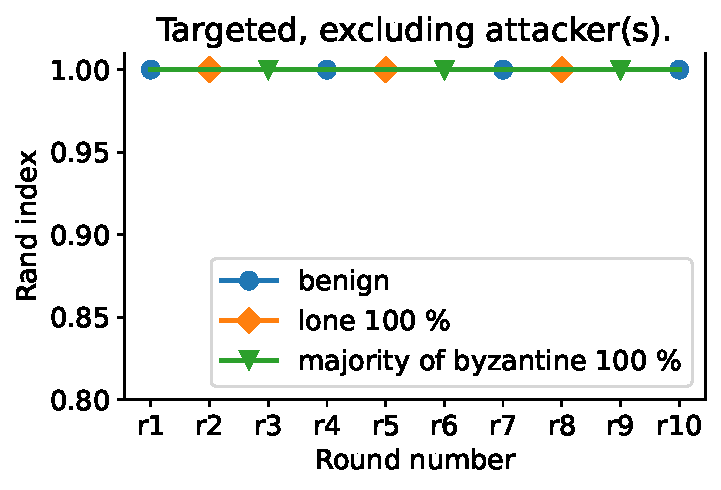
\includegraphics[width=0.45\linewidth]{figures/clustering/targeted_rand_no_attackers.pdf}
    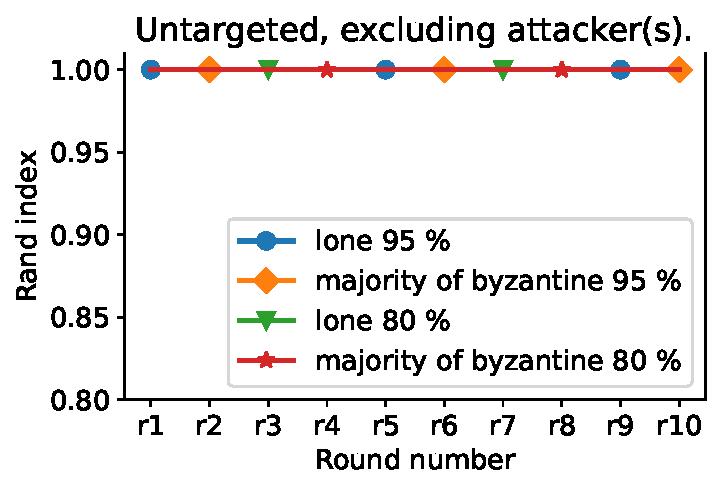
\includegraphics[width=0.45\linewidth]{figures/clustering/untargeted_rand_no_attacker.pdf}
    
    \caption{Comparison of the clustering results with a partition of participants that doesn't include the attackers. The constant rand index of 1 under different attack scenario mean that benign participants are correctly grouped according to the origin of their data in all scenario.}
    \label{fig:rand_no_attackers}
  \end{subfigure}
  \hfill 
    \begin{subfigure}{\columnwidth}
    \centering 
    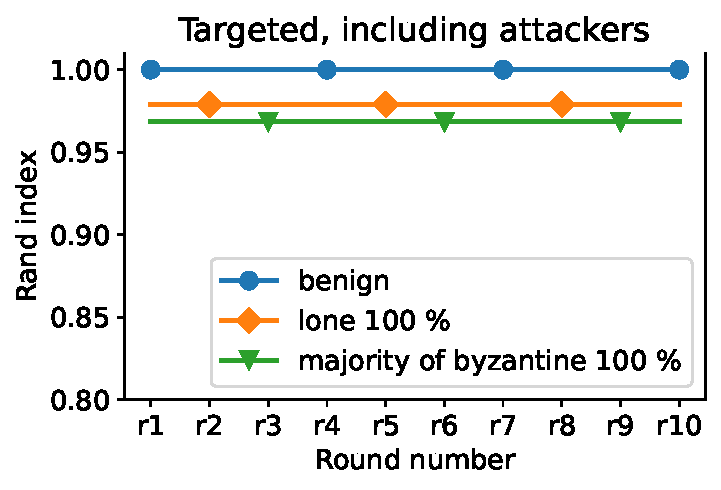
\includegraphics[width=0.45\linewidth]{figures/clustering/targeted_rand_attackers_separated.pdf}
    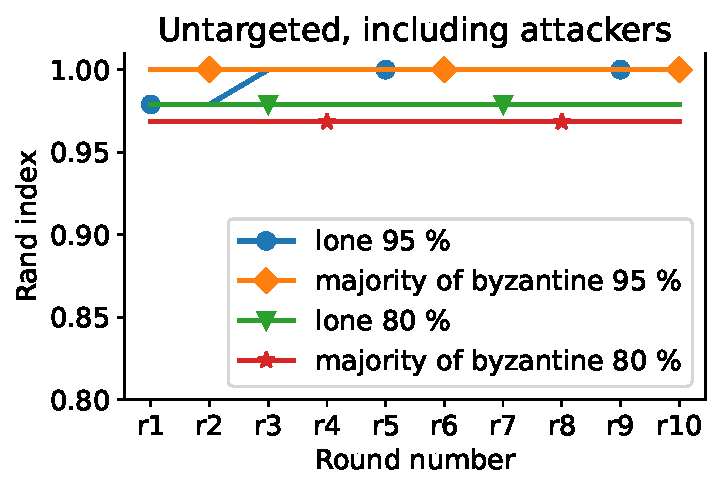
\includegraphics[width=0.45\linewidth]{figures/clustering/untargeted_rand_attackers_separated.pdf}
    \caption{The partition used for comparison include attackers and place them in their own group. For the loudest untargeted attacks, this is the observed behavior. In the others cases attackers are grouped with benign. }
    \label{fig:rand_attackers_separated}
  \end{subfigure}
  \hfill  
  \caption{Rand index evaluation of the clustering results under different attack scenario.}
  \label{fig:rand_clustering}
\end{figure*}
The comparison with this first partition is illustrated in \Cref{fig:rand_no_attackers}, we can see that benign participants are perfectly grouped according to their original dataset. 
This is true in the benign scenario, when there is no attacker, and more generally for the different attack scenarios. 
Another interesting result from clustering is that the loudest attackers are placed in their own cluster. 
In \Cref{fig:rand_attackers_separated} we see that for untargeted attacks with at least 95\% of poisoned data the obtained partition perfectly match the one where attackers are separated. %both for single and group of attackers.
For targeted attacks or untargeted attacks with lower poisoning rate, however, attackers are grouped with the benign participants from the dataset they are poisoning. 
In summary, our clustering approach directly place the noisiest attacks in their own cluster, regardless of their numbers, thus negating their effect. 
It then reliably groups participants according to their original dataset, creating the necessary conditions for the reputation system to manage more discrete attacks. 

%We used the following hyperparameters for the clustering: distance were measured using cosine~similarity, see \Cref{eq:cosin_sim} and the hierarchical clustering threshold is equal to 1/4th of the mean initial inter-distance. 

% Scénarios avec des attaques. 
\subsubsection{Reputation system\label{sec:eval.results.reput}}
The goal of the reputation system is to weight participants in each cluster. 
It should minimize the weight of attackers without impacting too much the weight of benign participants. 

\begin{figure*}[t]
    \centering
     \begin{subfigure}{0.45\columnwidth}
    \centering 
    \includegraphics[width=\linewidth]{figures/reput/benign_non_exploded.pdf}
    \caption{Benigns only}
    \label{fig:benign_targeted_non_exploded}
  \end{subfigure}
    \hfill 
     \begin{subfigure}{0.45\columnwidth}
    \centering 
    \includegraphics[width=\linewidth]{figures/reput/lone_loud_non_exploded.pdf}
    \caption{Lone attacker}
    \label{fig:lone_loud_non_exploded}
  \end{subfigure}
    \hfill 
    \begin{subfigure}{0.45\columnwidth}
    \centering 
    \includegraphics[width=\linewidth]{figures/reput/byzantine_minority_loud_non_exploded.pdf}
    \caption{Minority of Byzantines}
    \label{fig:byzantine_minority_loud_non_exploded}
  \end{subfigure}
    \hfill 
  \begin{subfigure}{0.45\columnwidth}
    \centering 
    \includegraphics[width=\linewidth]{figures/reput/byzantine_majority_loud_non_exploded.pdf}
    \caption{Majority of Byzantines}
    \label{fig:byzantine_majority_loud_non_exploded}
  \end{subfigure}
    \caption{Reputation weights for the participants of the poisoned cluster on targeted attacks.}
    \label{fig:non_exploded_reputation}
\end{figure*}


\begin{figure}[t]
%\begin{minipage}{.49\textwidth}
  \centering 
  \begin{subfigure}{0.49\columnwidth}
    \centering 
    \includegraphics[width=\linewidth]{figures/reput/byzantine_minority_loud_exploded.pdf}    \caption{Targeted minority of Byzantines, exploded.}
    \label{fig:targeted_byzantine_minority_exploded_reputation}
  \end{subfigure}
   \begin{subfigure}{0.49\columnwidth}
    \centering 
    \includegraphics[width=\linewidth]{figures/reput/untargeted_byzantine_minority_stealth_0_9.pdf}    
    \caption{Untargeted, 90\% poisoning, non exploded.}
    \label{fig:untargeted_byzantine_minority_non_exploded_reputation}
  \end{subfigure}
  \caption{Effect of exploding weights on targeted attackers, untargeted attackers}
  \label{fig:exploding_weights}
%\end{minipage}
\end{figure}
%\hfill
\begin{figure}[t]
%\begin{minipage}{.49\textwidth}
  \centering 
  \begin{subfigure}{0.49\columnwidth}
    \centering 
    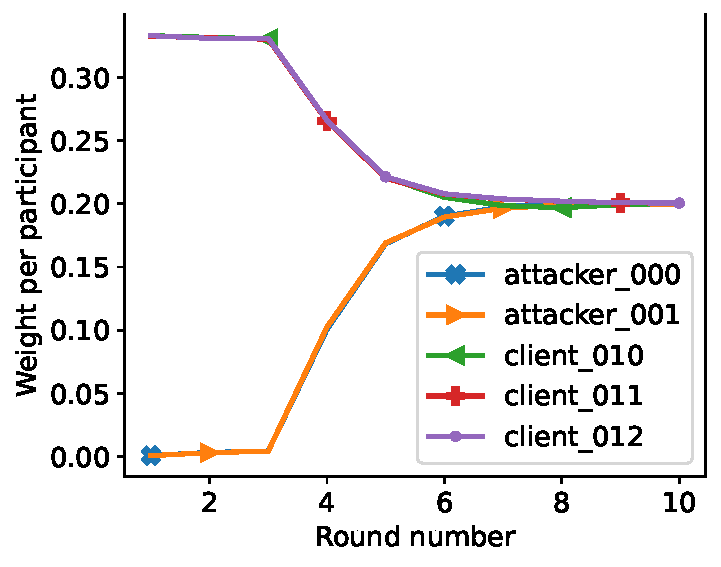
\includegraphics[width=\linewidth]{figures/reput/redemption_byzantine_min.pdf}    
    \caption{100\% poisoning until round 3, attackers become benign afterwards.}
    \label{fig:redemption_byzantine_min}
  \end{subfigure}
 \begin{subfigure}{0.49\columnwidth}
    \centering 
    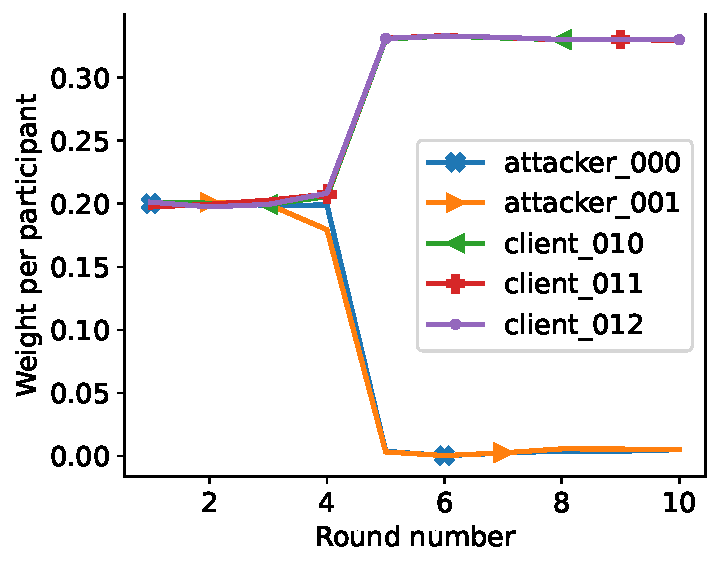
\includegraphics[width=\linewidth]{figures/reput/increment_byzantine_min.pdf}    \caption{Attackers begin as benign and add 20\% poisoning per round starting on round 3.}
    \label{fig:increment_byzantine_min}
  \end{subfigure}
  \caption{Weight per participants in the targeted cluster, attack is targeted and is done by a minority of byzantine.}
  \label{fig:redemption_decrease}
%\end{minipage}
\end{figure}

\Cref{fig:non_exploded_reputation} presents the weight $\weight$ given by the reputation system to participants inside a single cluster. 
\Cref{fig:benign_targeted_non_exploded} illustrates that there is little difference between benign participants of the same cluster.
In the case of a scenario with a single attacker (\Cref{fig:lone_loud_non_exploded}) or a minority of Byzantines (\Cref{fig:byzantine_minority_loud_non_exploded}), their weight is reduced compared to benign participants: the reputation system successfully identifies them as outliers. %Petite phrase pour dire qu'on a moins d'écart entre les sybils et le bénin que l'attaquant seul ?
Finally, when Byzantines attackers becomes the majority (\Cref{fig:byzantine_majority_loud_non_exploded}), they gain precedence in weight and benign participants' weight drop. 
This is expected: by construction, the reputation system favors the opinion of the majority in case of disagreement.  

The drawback of the reputation presented in \Cref{fig:non_exploded_reputation} is that the absolute difference in weight between attackers and benign participants is small.  
Thus, it is required to further explode the weight before using them for the aggregation.
\Cref{fig:targeted_byzantine_minority_exploded_reputation} is the exploded counterpart of \Cref{fig:byzantine_minority_loud_non_exploded}.  
% TODO : section explosion des poids dans l'architecture.

As shown in \Cref{fig:untargeted_byzantine_minority_non_exploded_reputation} untargeted attacks, are tremendously easier to detect for the reputation system and their weight is already small even before being exploded. 

In~\Cref{fig:redemption_decrease} we control how the reputation system reacts to attackers that change their behavior overtime. 
The weights of the attackers that stopped their attack raise to the benign participants' in only a few rounds. 
The number of rounds it takes depends on the choice of the $\lambda$ history parameter. 
We chose to set it 0.3 for the experiments, a value that will tend to favor recent rounds over older ones.  
We also see this in~\Cref{fig:redemption_decrease}, after a first round where the poisoning isn't detected, the weight of the newly detected attacker is quickly adjusted. 
% Petit § sur l'empoisonnement progressif. 
% Je veux retenir que : 
% 1. Le système est capable de suivre un changement de comportement. 
% Progressif dans le fait de refaire confiance. 
% Brutale mais avec un peu de délai dans la réduction du poids. 

% Exploding the weight + effets de l'explosion sur les bénins.

%  Présentations des cas de base : bénins, lone, sybils_min, sybils_majority en loud voir les effets et les limites. 

% Présentation de quelques cas limites : increase, decrease. 

%Idéalement test de l'efficacité du système avec et sans historique (ou en faisant varier le paramètre alpha) dans les cas d'empoisonnement progressifs. 

% Montrer les effets de l'historique ? Peut-être pas indispensable car prends de la place sans être rapprochable à un cas d'usage réel.

%  
